\section{Materials and Methods}

\subsection*{Cow Husbandry}

The studied cows were housed in a free-stall barn at Virginia Tech Dairy Comlex at Kentland Farm in Virginia, USA. The cow handling and image capturing were conducted following the guidelines and approval of the Virginia Tech Institutional Animal Care and Use Committee (\#IACUC xxxxx).

\subsection*{Image Dataset}

The images in this study were collected using the Amazon Ring camera model Spotlight Cam Battery Pro (Ring Inc.), which offers a real-time video feed of dairy cows. Three cameras were installed in the barn: two at a height of 3.25 meters (10.66 feet) above ground covering an area of 33.04 square meters (355.67 square feet). One camera provided a top view while the other was angled approximately 40 degrees from the horizontal to offer a side view of the cows. These are hereafter referred to as \textit{the top-view camera} and \textit{the side-view camera}, respectively. A third camera, termed \textit{the external camera}, was set at a lower height of 2.74 meters (9.00 feet) and covered a larger area of 77.63 square meters (835.56 square feet). Positioned 10 degrees downward from the horizontal, it captured a challenging perspective prone to occlusions among cows.

Images were captured using an unofficial Ring Application Programming Interface (API) \citep{greif_dgreifring_2024}, configured to record a ten-second video clip every 30 minutes continuously for 14 days. Since the image quality relies on the camera's internet connection, which was occasionally unstable, some images were found to be tearing or unrecognizable. Hence, the resulting dataset was manually curated for consistent quality, comprising 504 images from \textit{the top-view camera}, 500 from \textit{the side-view camera}, and 250 from \textit{the external camera}. These images were futher categorized based on the lighting conditions: for \textit{the top-view camera}, 296 images were captured during daylight, 118 in the evening under artificial lighting, and 90 as near-infrared images without artificial light. From \textit{the side-view camera}, 113 images were taken in the evening, and 97 as near-infrared images. All images from \textit{the external camera} were captured during the day. The image examples were shown Figure ~\ref{fig:dataset}

\begin{figure}[h]
    \centering
    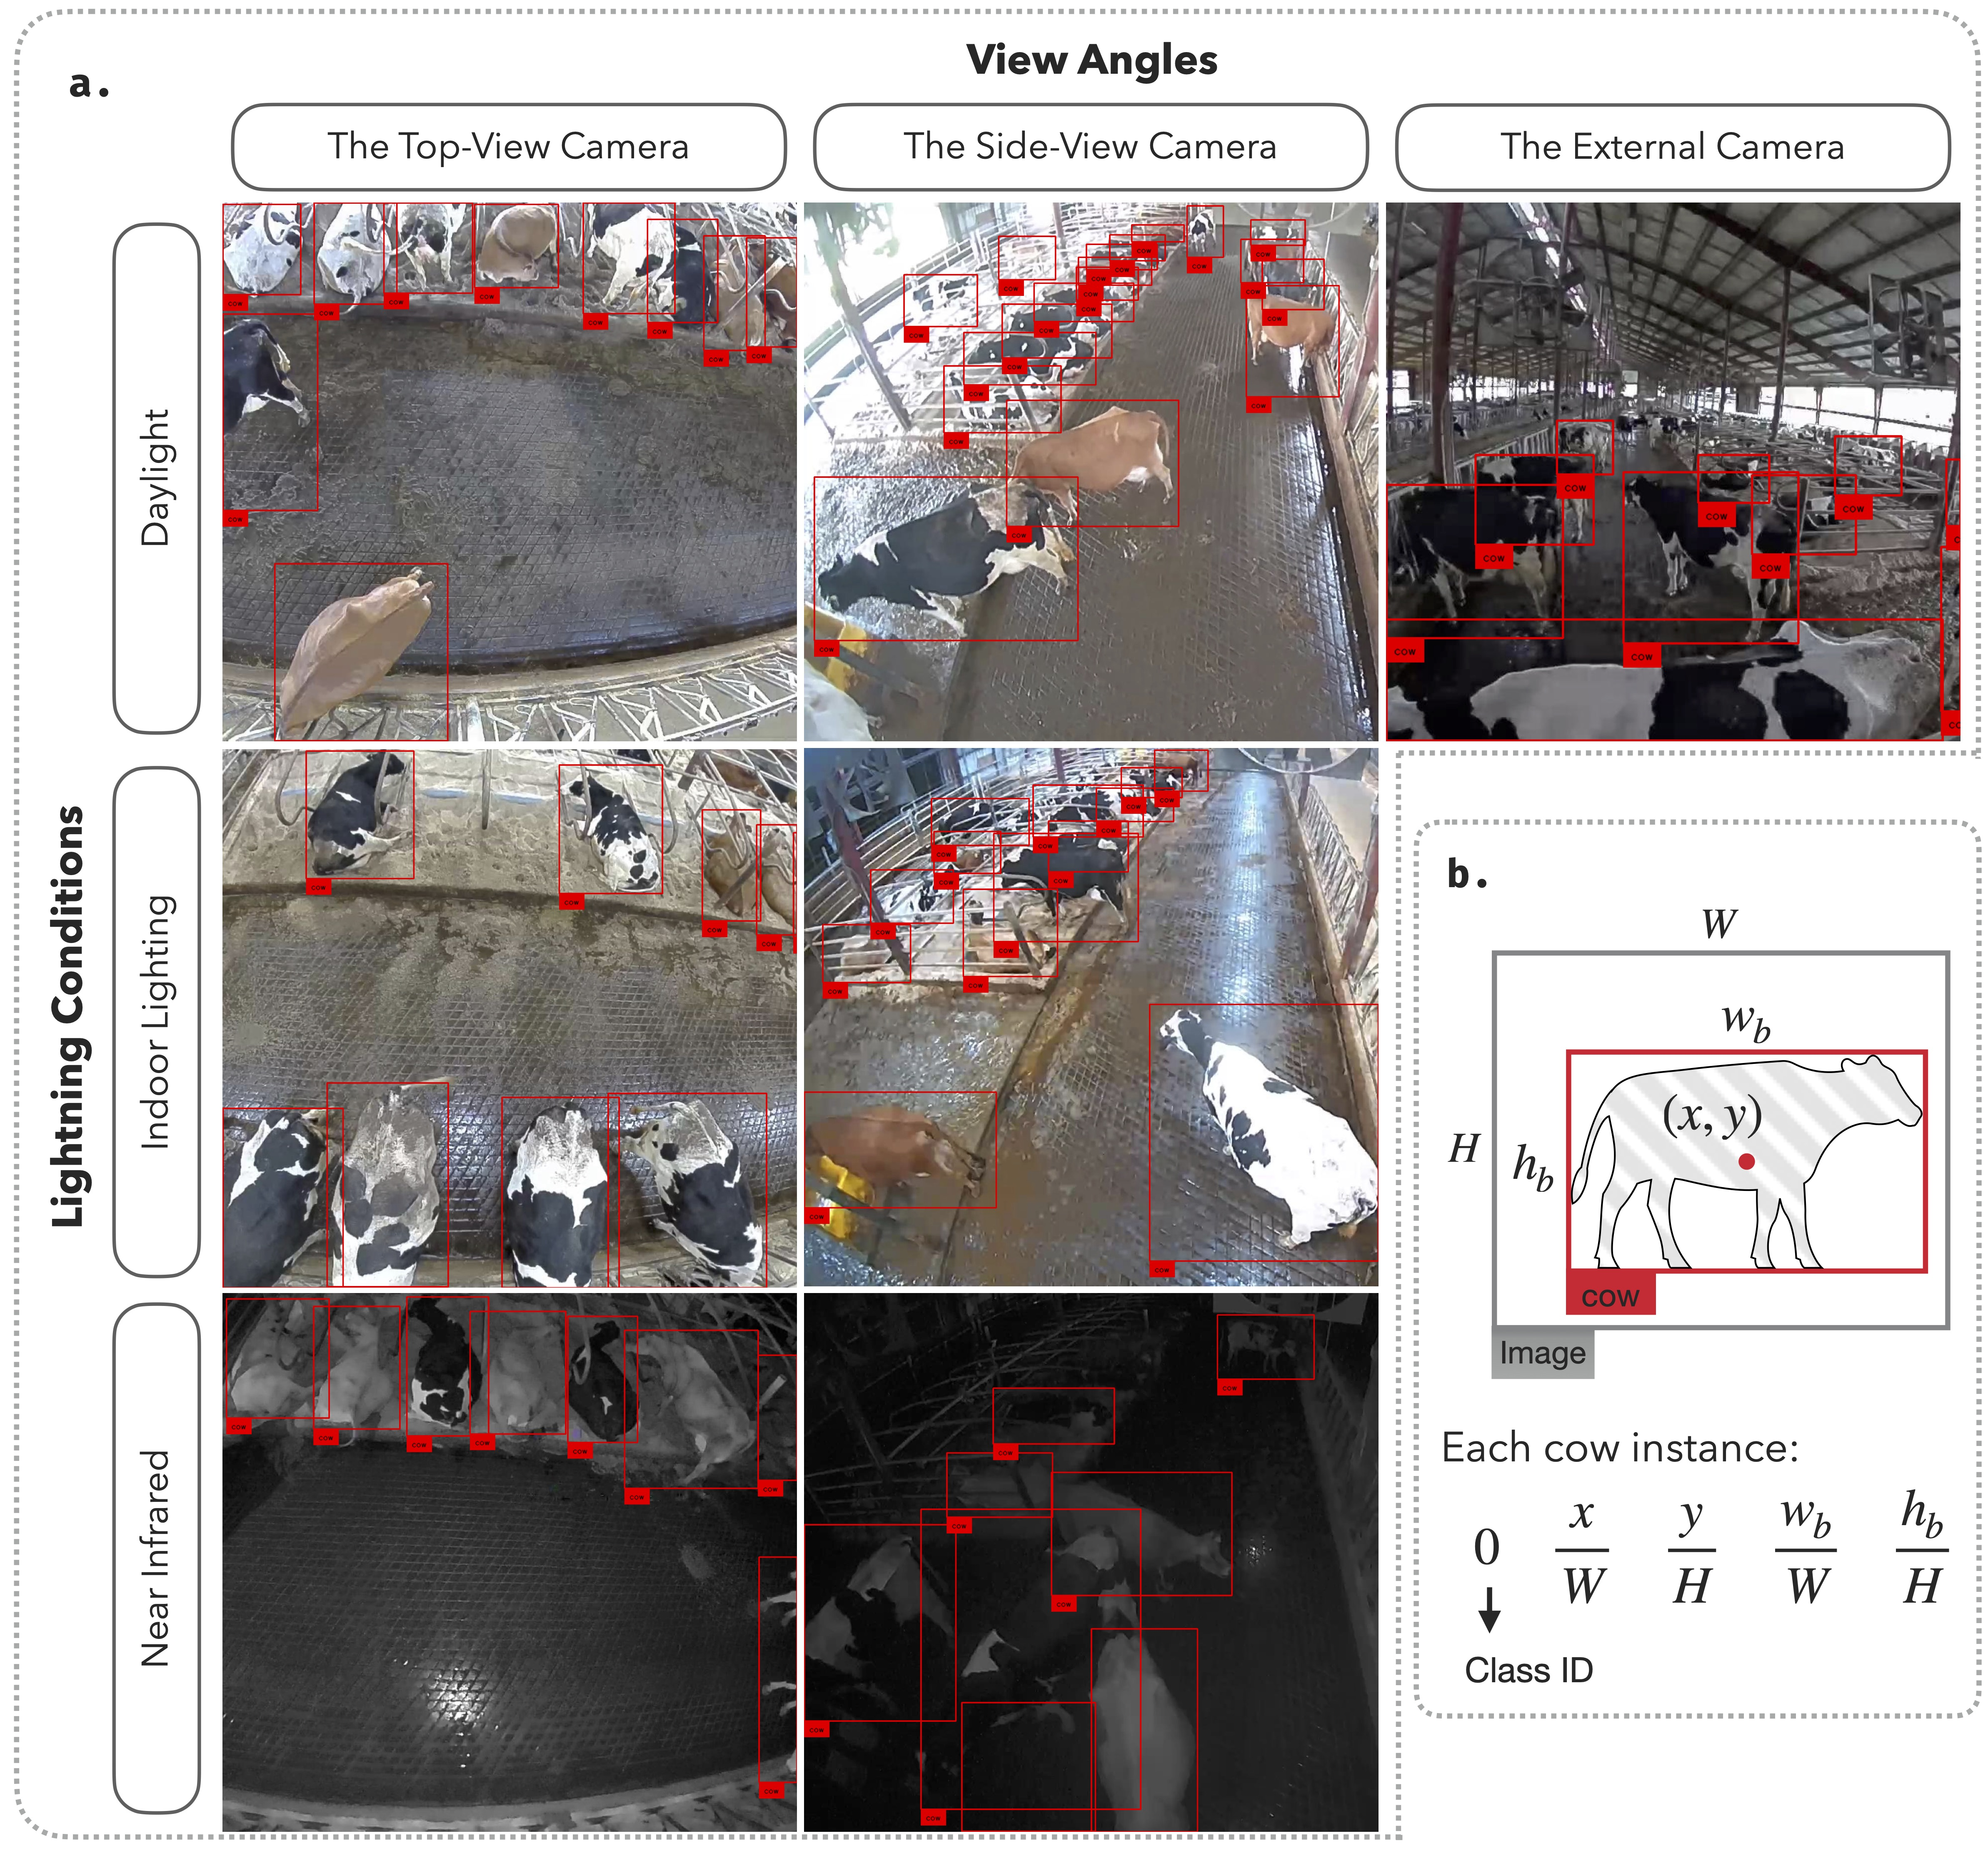
\includegraphics[width=1\textwidth]{figure_1.jpg}
    \caption{Examples of the annotated images.}
    \label{fig:dataset}
\end{figure}

The image annotations were conducted using an online platform, Roboflow \citep{}, to define cow positions in the images. The bounding boxes were manually drawn to enclose the cow contours, providing the coordinates of the top-left corners and the width and height of the boxes. If cows were partially occluded, the invisible parts were infered based on the adjacent visible parts. If the cow position was too far from the camera and make the important body features, such as head, tail, and legs, unrecognizable, the cow was excluded from the dataset. The final annotations were saved in the YOLO format \citep{}, where annotations were stored in a text file with one row per cow in the image, each row containing the cow's class, center coordinates, width, and height of the bounding box. The graphical representation of the annotated images was shown in Figure XXX.

\subsection*{Model Training}

The model training was implemented using the python library Ultralytics \citep{}. The model hyperparameters were set by the default values in the library. The training epochs were set to 100, and the batch size was set to 16. The implemented data augmentation include randomly changing the image color hue, saturation, and exposure to improve the model generalizing to different lighting conditions. Geometry augmentation was also applied by randomly flipping the images horizontally, copying and pasting to mix up object instances across multiple images to increase data diversity, and randomly scaling the images to simulate different distances between the camera and the cows. The details of the hyperparameters were shown in ~\ref{tab:hyperparameters}. The training was conducted on an NVIDIA A100 GPU (NVIDIA, USA) with 80GB video memory provided by Advanced Research Computing at Virginia Tech.


\subsection*{Model Evaluation}

The examined YOLO models are object detection models that return positions of detected objects (i.e., cows in this study) for the evaluated images. The detections are represented by a list of boudning boxes. Regardless of specific procedures among YOLO variants for computational efficiency, such as YOLOv8 that integrate objectness scores and conditional class probabilities into a single confidence score, each detection generally consist of $4+c$ elements: the xy-coordinates, width, and height of the bounding box, and the $c$ confidence scores indicating the probability of the object belonging to each of the $c$ classes. The class with the highest confidence score is considered the predicted class of the object. To evaluate the model performance, two aspects are considered: the localization accuracy and the classification accuracy. The localization accuracy is measured by the Intersection over Union (IoU) between the predicted bounding box and the ground truth bounding box. On the other hand, the classification accuracy is measured by the precision and recall given the confidence threshold. If the confidence score of a detection is higher than the threshold, the detection is considered as a positive detection. Otherwise, the detection is neglected. Combining the localization and classification accuracy, the mean Average Precision ($mAP$) averaged the area under the precision-recall curve across all the classes. The curve is generated by varying the confidence threshold from 0 to 1 given a IoU threshold. In this study, four metrics were used in the evaluation: the precision and recall at the confidence threshold of 0.25 and IoU threshold of 0.5, the mAP at the IoU threshold of 0.5 (noted as $\text{mAP@{0.5}}$), and the averaged mAP at varying IoU thresholds ranging from 0.5 to 0.95 (noted as $\text{mAP@{0.5:0.95}}$.)


\subsection*{Study 1: Benchmarking Model Generalization Across Different Environmental Conditions}

To compare the performance drop between different view angles and lighting conditions, we designed a cross-testing strategy where models were trained on one dataset configuration and tested on another. There are five training configurations in this study:

\begin{itemize}
    \item \textbf{Baseline:} The model was trained and evaluated on the dataset characterized for all the conditions including top-view, side-view, daylight, evening, and near-infrared images. The images were not overlapped between the training and evaluation sets.
    \item \textbf{Top2Side:} The model was trained on the top-view images and evaluated on the side-view images.
    \item \textbf{Side2Top:} The model was trained on the side-view images and evaluated on the top-view images.
    \item \textbf{Day2Night:} The model was trained on the daylight images and evaluated on the evening images, including both artificial lighting and near-infrared images.
    \item \textbf{External:} The model was trained on images collected by the top-view and side-view cameras and evaluated on the external camera images.
\end{itemize}


\begin{figure}[h]
    \centering
    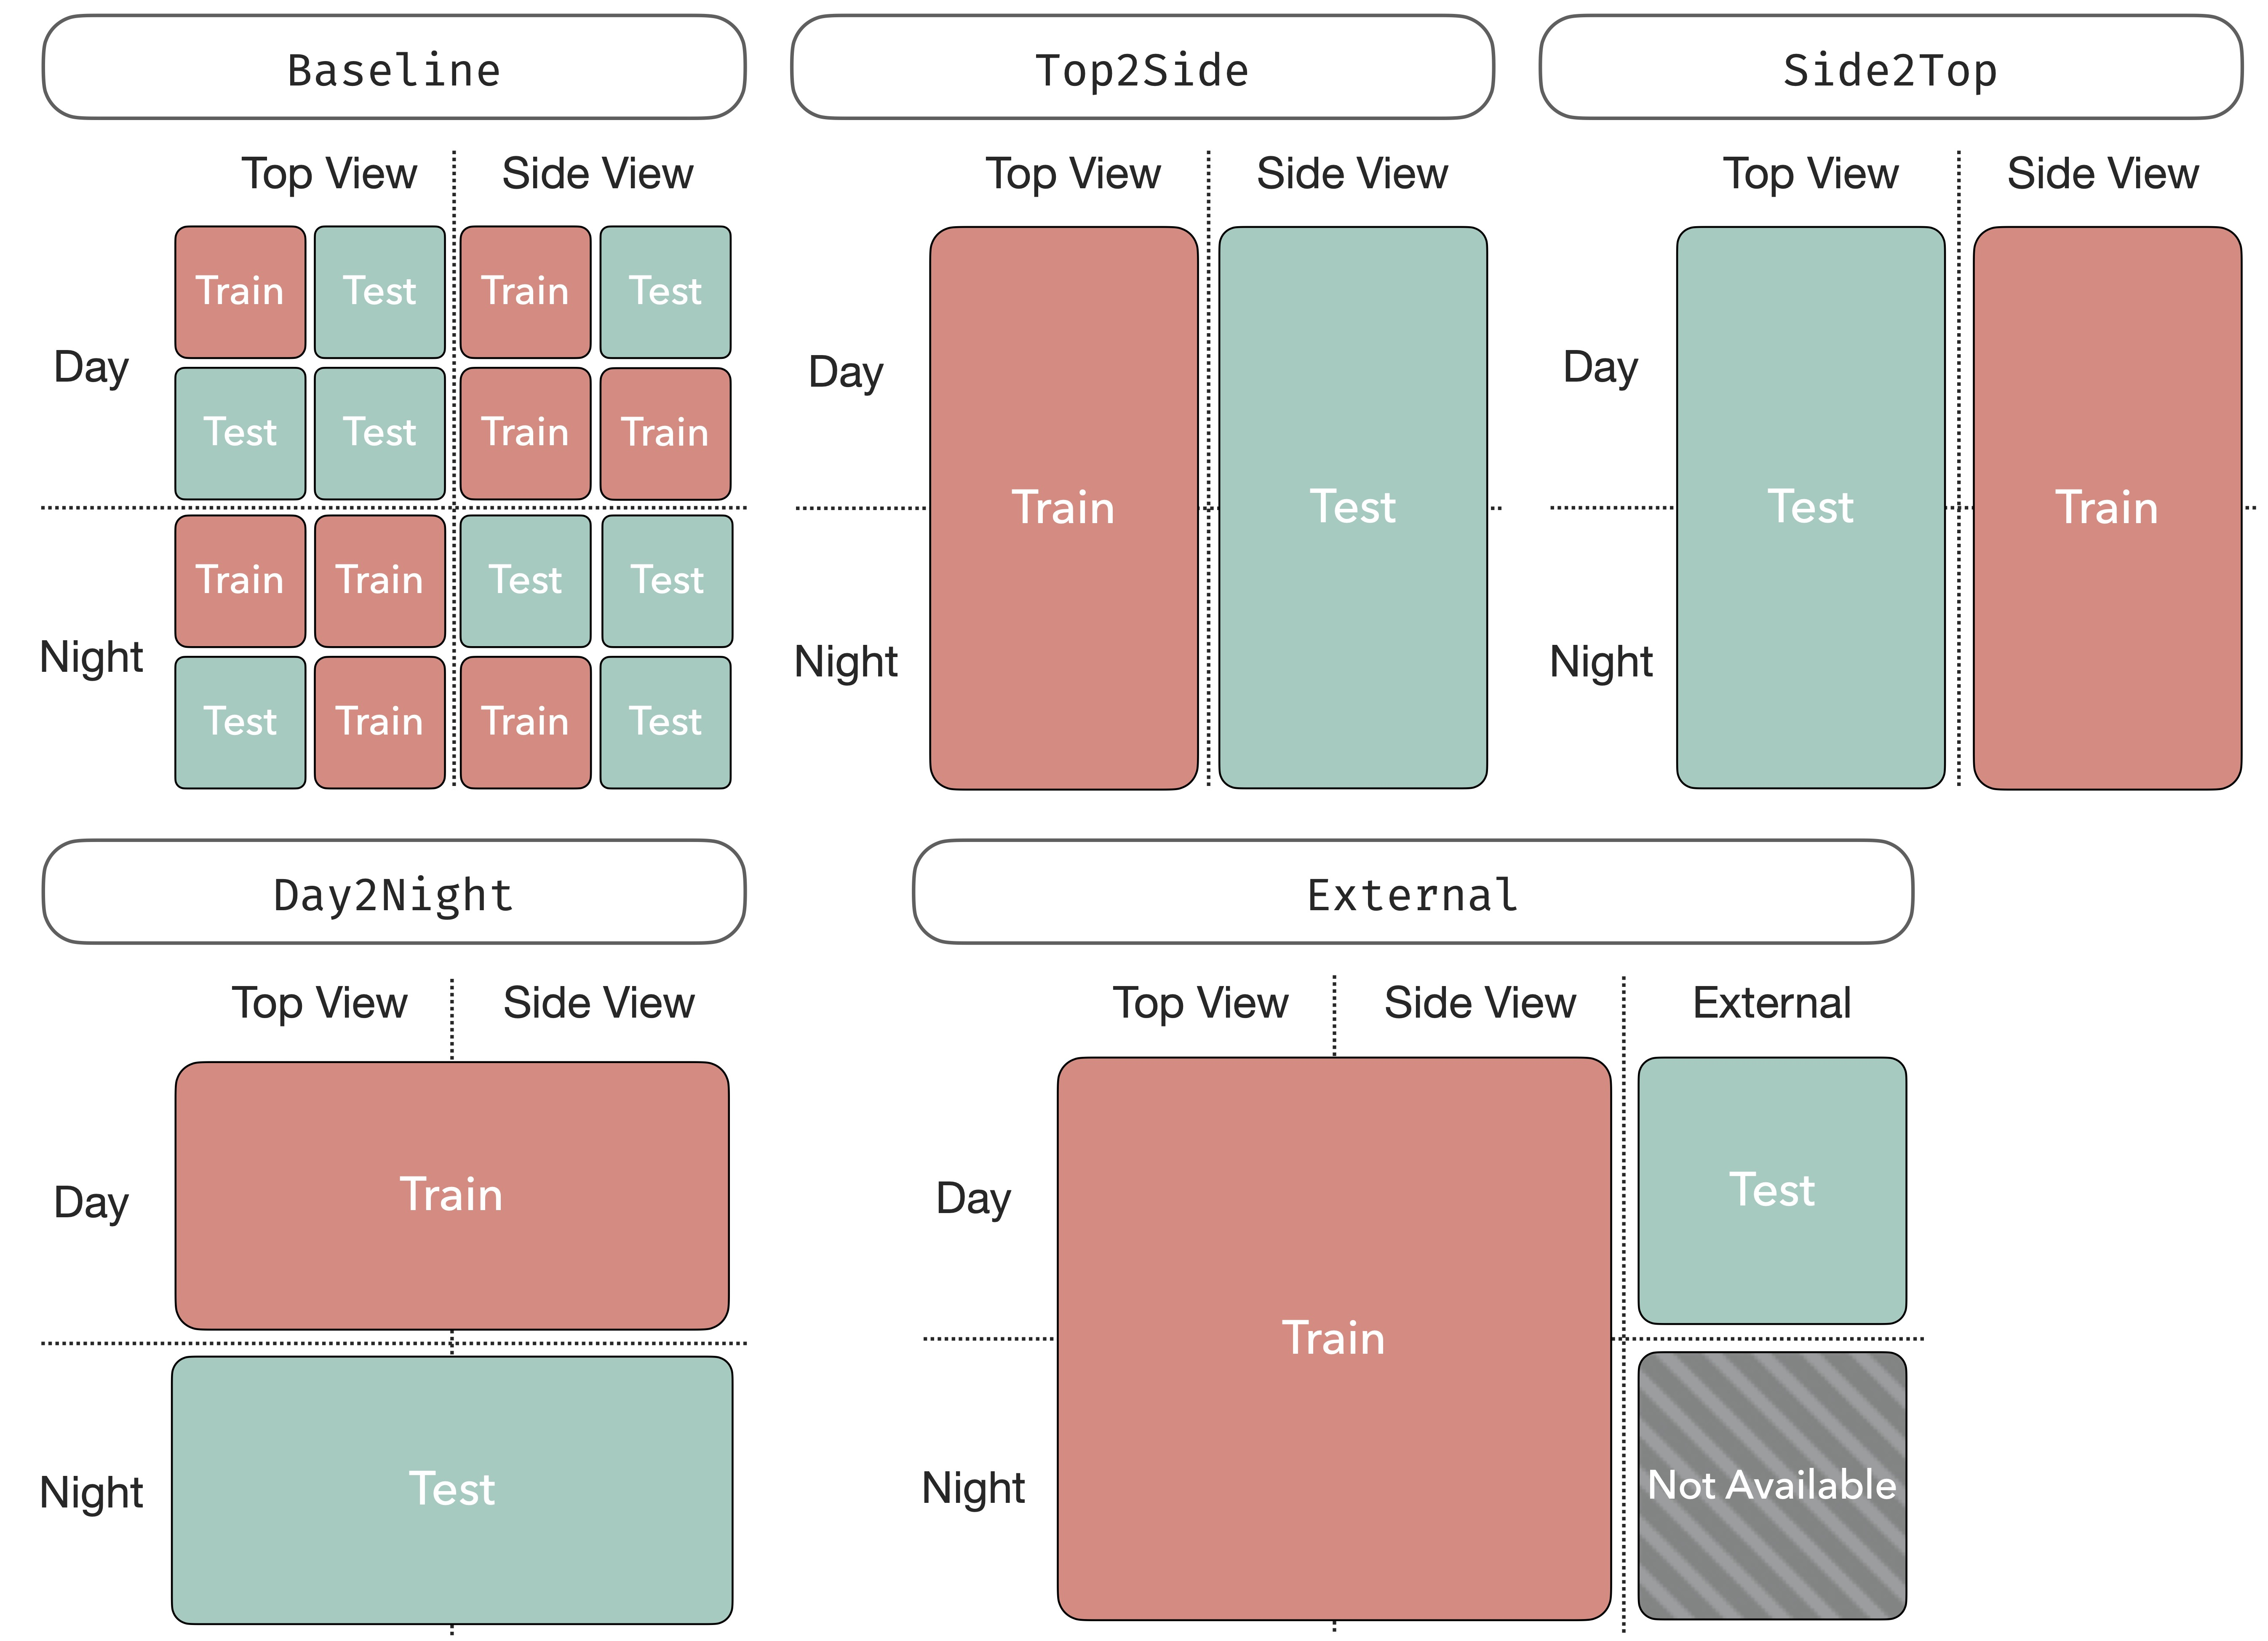
\includegraphics[width=0.8\textwidth]{figure_2.jpg}
    \caption{Examples of the annotated images.}
    \label{fig:splits}
\end{figure}

To study how the training sample size affects the model performance in each configuration, the testing set in the cross-validation was first fixed to the same 100 images. Then, the training set size was altered iteratively from 16 to 512 images with a step size of doubling the sample size. Each training sample size was repeated 50 times with different random seeds to ensure the robustness of the results. The YOLOv9e, which is the most capable model in the YOLO family to date according to the performance on the COCO datset, was used as the base model for this study.


\subsection*{Study 2: The correlation between model complexity and performance on the tasks of localizing cows}

To investigate whether the model performance increases with the model complexity, five YOLO-family models were investigated in thie study. Three of the models were selected from the YOLOv8 family: YOLOv8n, YOLOv8m, and YOLOv8x. All the YOLOv8 models shared the similar model architecture. The differences among the variants are deepen multipler, width multipler, and ratio factor, which collectively determine their parameter counts of 3.2 millions (m), 25.9m, and 68.2m, respectively. The deepen multipler determine how many convolutional layers are repeated in a C2F module, which is the novelty of the YOLOv8. The width multipler and ratio factor collectively specify the channel numbers in the convolutional operations. Correspondingly, the YOLOv8n, YOLOv8m, and YOLOv8x were defined by the deep multipliers of 0.33, 0.67, and 1.0, respectively. The width multipliers, are 0.25, 0.75, and 1.25, while the ratio factor are 2.0, 1.5, and 1.0 \citep{}. These variations enable the models to achieve different balances between computational efficiency and accuracy. The remaining two models were YOLOv9c and YOLOv9e, which are the latest models in the YOLO family and are with parameter counts of 25.6M and 58.2M, respectively.  Unlike YOLOv8 models, these models have slightly different backbone architectures. Although the majority of the model components between YOLOv9c and YOLOv9e are the same, they primarily differ in their layer counts, module complexities, and depth configurations. YOLOv9c has 618 layers and uses simpler modules, resulting in a more efficient model with lower computational demands. Conversely, YOLOv9e has 1225 layers and employs more advanced modules \citep{}. All models were trained on 500 images in each of four configurations described in Study 1.

In addition to the model performance, the computing speed was also evaluated. The training speed was recorded in seconds per 100 epochs, and the inference time was recorded as frames per second (FPS) on both the CPU and GPU (Apple M1 Max chip, Apple Inc.) The relationship between the model complexity and the time consumption was analyzed to provide insights into the trade-off between the model performance and the computational cost.

\subsection*{Study 3: Assessing the advantages of using fine-tuned model over the pre-trained model as initial model weights}

Most models are released with the pre-trained weights, which were obtained from the large dataset containing millions of object instances (e.g., COCO\citep{} and ImageNet\citep{}). The pre-trained models have general capability in recognizing common objects such as vehicles, animals, and household items. When the model is required to recognize specific objects (i.e., cows in this study), having a model trained on a smaller but specific dataset is expected to have a better performance. However, such advantages may not necessarily persist as the training sample size increases. Having equally enough samples for both the pre-trained and fine-tuned models could diminish the performance gap between the two models. To investigate this hypothesis, this study evaluated the performance of the fine-tuned models with two different initial weights. The first initial weight was the default weights from the pre-trained model on the COCO dataset, while the second initial weight was the weights from the fine-tuned model on the opposite view angle. The cross-validation settings were described in the Table ~\ref{tab:configuration}.

\begin{table}[h]
    \centering
    \begin{tabular}{ccl}
        \toprule
        \textbf{Case} &\textbf{Finetuning Data Sources} & \textbf{Initial Weights} \\
        \midrule
        1 &Top-View Camera & COCO (default) \\
        2 &Top-View Camera & Side-View Camera \\
        3 &Side-View Camera & COCO (default) \\
        4 &Side-View Camera & Top-View Camera \\
        \bottomrule
    \end{tabular}
    \caption{Train and test data configurations with and initial weight criteria.}
    \label{tab:configuration}
\end{table}

The backbones of the all models (i.e., YOLOv8n, YOLOv8m, YOLOv8x, YOLOv9c, and YOLOv9e) were fine-tuned across different training sample sizes, which are 16, 32, 64, 128, 256, and 500. The goal was to determine whether the advantage of using the fine-tuned weights persist under the interaction between the model complexity and different fine-tuning samples. The performance of the models was evaluated using $\text{mAP@{0.5:0.95}}$.




